\subsection{Erdvės diskretizavimas}

Abiems skaitiniams modeliams naudosime tokiu pačiu principu sukonstruotą tinklelį. Jį sudarydami padaliname stačiakampę sritį $\Omega$ į $N\times M$ taškų, kurie yra nutolę vienas nuo kito fiksuotais atstumais $\Delta x$ ir $\Delta y$ atitinkamomis ašimis. Analogiškai, laiko intervalą $[0, T]$ padalinsime į $K + 1$ taškų, kurie vienas nuo kito yra nutolę tolygiais $\Delta t$ atstumais. Apibūdinta diskretų tinklelį galima užrašyti taip:

\begin{align}
    \omega_W&=\{ x_i : x_i = i\Delta x, \quad i=0, 1, \dots, N - 1 \} & \Delta x&=\frac{W}{N-1} \label{meshx}\\
    \omega_H&=\{ y_j : y_j = j\Delta y, \quad j=0, 1, \dots, M - 1 \} & \Delta y&=\frac{H}{M-1} \label{meshy}\\
    \omega_K&=\{ t_n : t_n = n\Delta t,\quad n=0, 1, \dots, K\} & \Delta t&=\frac{T}{K} \label{mesht}\\
	\omega&=\omega_W\times\omega_H\times\omega_K \label{mesh}
\end{align}

\begin{figure}[!h]
\centering
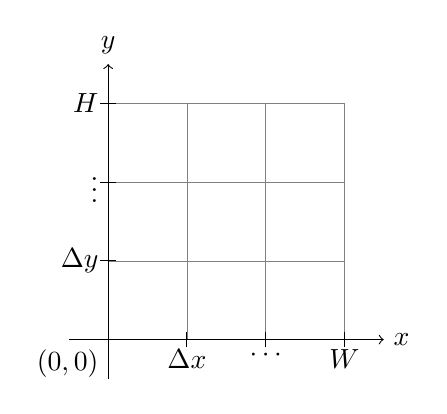
\begin{tikzpicture}
    
% Define the size of the cells
\def\Deltax{1} % Delta x size
\def\Deltay{1} % Delta y size
\def\Xmax{4} % Max X value
\def\Ymax{4} % Max Y value

% Draw the mesh
\foreach \x in {0,1,2} {
    \foreach \y in {0,1,2} {
        \draw[help lines] (\x*\Deltax,\y*\Deltay) grid (\x*\Deltax+\Deltax,\y*\Deltay+\Deltay);
    }
}

\node[below left] at (0,0) {$(0, 0)$};

% Draw axes
\draw[->] (-0.5,0) -- (3.5 *\Deltax,0) node[right] {$x$} ;
\draw[->] (0,-0.5) -- (0,3.5) node[above] {$y$};

% Add tick marks on x-axis with labels
\draw[shift={(1,0)}] (0,-0.1) -- (0,0.1);
\node[below] at (1, 0) {\(\Delta x\)};

\draw[shift={(2,0)}] (0,-0.1) -- (0,0.1);
\node[below] at (2, 0) {$\cdots$};

\draw[shift={(3,0)}] (0,-0.1) -- (0,0.1);
\node[below] at (3, 0) {$W$};

% Add tick marks on y-axis with labels

\draw[shift={(0,1)}] (-0.1,0) -- (0.1,0);
\node[left] at (0, 1) {$\Delta y$};
        
\draw[shift={(0,2)}] (-0.1,0) -- (0.1,0);
\node[left] at (0, 2) {$\vdots$};

\draw[shift={(0,3)}] (-0.1,0) -- (0.1,0);
\node[left] at (0, 3) {$H$};

\end{tikzpicture}
\caption{ Diskretizuota erdvė }
\end{figure}

\newpage